\documentclass[tikz,border=5pt]{standalone}

\usepackage{amsmath,amssymb}
\usetikzlibrary{arrows.meta,positioning,calc}

\begin{document}
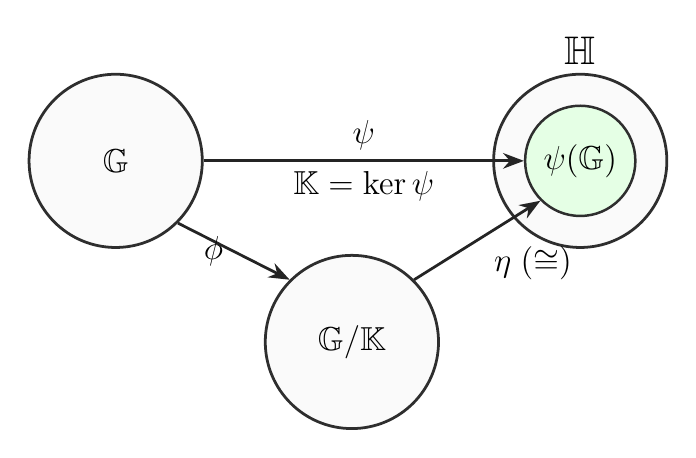
\begin{tikzpicture}[
  >=Stealth,
  every node/.style={font=\large},
  mainnode/.style={circle, draw=black!82, fill=black!2, line width=1pt, minimum size=22mm},
  imagenode/.style={circle, draw=black!82, fill=green!10, line width=.9pt, minimum size=14mm},
  map/.style={->, draw=black!86, line width=1pt},
  iso/.style={->, draw=black!86, line width=1pt}
]
  \node[mainnode] (G) at (0,1.25) {$\mathbb{G}$};
  \node[mainnode] (H) at (5.9,1.25) {};
  \node[font=\Large] at (5.9,2.65) {$\mathbb{H}$};
  \node[imagenode] (Im) at (5.9,1.25) {$\psi(\mathbb{G})$};

  \node[mainnode] (Q) at (3,-1.05) {$\mathbb{G}/\mathbb{K}$};

  \draw[map] (G.east) -- node[above] {$\psi$} node[below] {$\mathbb{K}=\ker\psi$} (Im.west);
  \draw[map] (G.south east) -- node[left] {$\phi$} (Q.north west);
  \draw[iso] (Q.north east) -- node[pos=.55, below right] {$\eta\;(\cong)$} (Im.south west);
\end{tikzpicture}
\end{document}
